%%%%%%%% ICML 2023 EXAMPLE LATEX SUBMISSION FILE %%%%%%%%%%%%%%%%%

\documentclass{article}

% Recommended, but optional, packages for figures and better typesetting:
\usepackage{microtype}
\usepackage{graphicx}
\usepackage{subfigure}
\usepackage{booktabs} % for professional tables

\usepackage{tikz}
% Corporate Design of the University of Tübingen
% Primary Colors
\definecolor{TUred}{RGB}{165,30,55}
\definecolor{TUgold}{RGB}{180,160,105}
\definecolor{TUdark}{RGB}{50,65,75}
\definecolor{TUgray}{RGB}{175,179,183}

% Secondary Colors
\definecolor{TUdarkblue}{RGB}{65,90,140}
\definecolor{TUblue}{RGB}{0,105,170}
\definecolor{TUlightblue}{RGB}{80,170,200}
\definecolor{TUlightgreen}{RGB}{130,185,160}
\definecolor{TUgreen}{RGB}{125,165,75}
\definecolor{TUdarkgreen}{RGB}{50,110,30}
\definecolor{TUocre}{RGB}{200,80,60}
\definecolor{TUviolet}{RGB}{175,110,150}
\definecolor{TUmauve}{RGB}{180,160,150}
\definecolor{TUbeige}{RGB}{215,180,105}
\definecolor{TUorange}{RGB}{210,150,0}
\definecolor{TUbrown}{RGB}{145,105,70}

% hyperref makes hyperlinks in the resulting PDF.
% If your build breaks (sometimes temporarily if a hyperlink spans a page)
% please comment out the following usepackage line and replace
% \usepackage{icml2023} with \usepackage[nohyperref]{icml2023} above.
\usepackage{hyperref}


% Attempt to make hyperref and algorithmic work together better:
\newcommand{\theHalgorithm}{\arabic{algorithm}}

\usepackage[accepted]{icml2023}

% For theorems and such
\usepackage{amsmath}
\usepackage{amssymb}
\usepackage{mathtools}
\usepackage{amsthm}

% if you use cleveref..
\usepackage[capitalize,noabbrev]{cleveref}

%%%%%%%%%%%%%%%%%%%%%%%%%%%%%%%%
% THEOREMS
%%%%%%%%%%%%%%%%%%%%%%%%%%%%%%%%
\theoremstyle{plain}
\newtheorem{theorem}{Theorem}[section]
\newtheorem{proposition}[theorem]{Proposition}
\newtheorem{lemma}[theorem]{Lemma}
\newtheorem{corollary}[theorem]{Corollary}
\theoremstyle{definition}
\newtheorem{definition}[theorem]{Definition}
\newtheorem{assumption}[theorem]{Assumption}
\theoremstyle{remark}
\newtheorem{remark}[theorem]{Remark}

% Todonotes is useful during development; simply uncomment the next line
%    and comment out the line below the next line to turn off comments
%\usepackage[disable,textsize=tiny]{todonotes}
\usepackage[textsize=tiny]{todonotes}


% The \icmltitle you define below is probably too long as a header.
% Therefore, a short form for the running title is supplied here:
\icmltitlerunning{Project Report Template for Data Literacy 2023/24}

\begin{document}

\twocolumn[
\icmltitle{My Data Literacy Project\\ (Replace this with your Project Title)}

% It is OKAY to include author information, even for blind
% submissions: the style file will automatically remove it for you
% unless you've provided the [accepted] option to the icml2023
% package.

% List of affiliations: The first argument should be a (short)
% identifier you will use later to specify author affiliations
% Academic affiliations should list Department, University, City, Region, Country
% Industry affiliations should list Company, City, Region, Country

% You can specify symbols, otherwise they are numbered in order.
% Ideally, you should not use this facility. Affiliations will be numbered
% in order of appearance and this is the preferred way.
\icmlsetsymbol{equal}{*}

\begin{icmlauthorlist}
\icmlauthor{Sumitrra Bala Subramaniam}{equal,first}
\icmlauthor{Jiha Kim}{equal,second}
\icmlauthor{Frederik Panse}{equal,third}
\icmlauthor{Kim Isabella Zierahn}{equal,fourth}
\end{icmlauthorlist}

% fill in your matrikelnummer, email address, degree, for each group member
\icmlaffiliation{first}{Matrikelnummer 6642271, sumitrra.bala-subramaniam@student.uni-tuebingen.de, MSc Quantitative Data Science Methods}
\icmlaffiliation{second}{Matrikelnummer 6640082, jiha.kim@student.uni-tuebingen.de, MSc Quantitative Data Science Methods}
\icmlaffiliation{third}{Matrikelnummer 5810899, frederik.panse@student.uni-tuebingen.de, MSc Quantitative Data Science Methods}
\icmlaffiliation{fourth}{Matrikelnummer 6635183, kim-isabella.zierahn@student.uni-tuebingen.de, MSc Quantitative Data Science Methods}

% You may provide any keywords that you
% find helpful for describing your paper; these are used to populate
% the "keywords" metadata in the PDF but will not be shown in the document
\icmlkeywords{Machine Learning, ICML}

\vskip 0.3in
]

% this must go after the closing bracket ] following \twocolumn[ ...

% This command actually creates the footnote in the first column
% listing the affiliations and the copyright notice.
% The command takes one argument, which is text to display at the start of the footnote.
% The \icmlEqualContribution command is standard text for equal contribution.
% Remove it (just {}) if you do not need this facility.

%\printAffiliationsAndNotice{}  % leave blank if no need to mention equal contribution
\printAffiliationsAndNotice{\icmlEqualContribution} % otherwise use the standard text.

\begin{abstract}
Put your abstract here. Abstracts typically start with a sentence motivating why the subject is interesting. Then mention the data, methodology or methods you are working with, and describe results. 
\end{abstract}

\section{Introduction}\label{sec:intro}
If a group of Tübinger students would want to take a trip to Frankfurt (Main) by train, there are many possible routes to take. Would they be able to decide beforehand on the most reliable route and the best time to go?

When traveling from one place to another by Deutsche Bahn, passengers often can't rely on arriving at their destination at the scheduled time. Even though real-time train delay is provided by the Deutsche Bahn, informing travelers about current delays, passengers don't have any information about the delay beforehand. Previous studies often focused on predicting train delay \cite{predtraindelay}. Our goal is to identify the most reliable train route going from Stuttgart to Frankfurt (Main).

We are working with \href{https://data.deutschebahn.com/dataset/ist-verkehrsdaten-der-db-cargo-auf-bst8-ebene.html}{train delay data} provided by the Deutsche Bahn, that consists of stations and stops that measured the number of trains and minutes of delay of all trains passing by in 2016. We are also using the corresponding \href{https://data.deutschebahn.com/dataset/betriebsstellen-gueterverkehr.html}{directory of operating sites} and \href{https://data.deutschebahn.com/dataset/betriebsstellen-gueterverkehr.html}{geographical route data} for our analyses.

To analyze the most reliable route going from Stuttgart to Frankfurt (Main), we followed two approaches: route optimization and analysing external influences. The first approach is to find all possible routes going from Stuttgart to Frankfurt (Main) and then identifying the route with the least mean delay (i.e., the most reliable route). The second approach is to investigate whether the day of the week, month, season, or holiday impact the delay.

Our study aims to fill a gap in train delay research by shifting the focus from predicting delays to informing passengers beforehand about the most reliable route and the best time to go. This enables passengers to make informed decision about their journeys. We aim to provide travelers with information, so that they can pick the optimal route with confidence and reliability.

Motivate the problem, situation or topic you decided to work on. Describe why it matters (is it of societal, economic, scientific value?). Outline the rest of the paper (use references, e.g.~to \Cref{sec:methods}: What kind of data you are working with, how you analyse it, and what kind of conclusion you reached. The point of the introduction is to make the reader want to read the rest of the paper.

\section{Data and Methods}\label{sec:methods}

In this section, describe \emph{what you did}. Roughly speaking, explain what data you worked with, how or from where it was collected, it's structure and size. Explain your analysis, and any specific choices you made in it. Depending on the nature of your project, you may focus more or less on certain aspects. If you collected data yourself, explain the collection process in detail. If you downloaded data from the net, show an exploratory analysis that builds intuition for the data, and shows that you know the data well. If you are doing a custom analysis, explain how it works and why it is the right choice. If you are using a standard tool, it may still help to briefly outline it. Cite relevant works. You can use the \verb|\citep| and \verb|\citet| commands for this purpose \citep{mackay2003information}.

% This is the template for a figure from the original ICML submission pack. In lecture 10 we will discuss plotting in detail.
% Refer to this lecture on how to include figures in this text.
% 
% \begin{figure}[ht]
% \vskip 0.2in
% \begin{center}
% \centerline{\includegraphics[width=\columnwidth]{icml_numpapers}}
% \caption{Historical locations and number of accepted papers for International
% Machine Learning Conferences (ICML 1993 -- ICML 2008) and International
% Workshops on Machine Learning (ML 1988 -- ML 1992). At the time this figure was
% produced, the number of accepted papers for ICML 2008 was unknown and instead
% estimated.}
% \label{icml-historical}
% \end{center}
% \vskip -0.2in
% \end{figure}

\section{Results}\label{sec:results}

In this section outline your results. At this point, you are just stating the outcome of your analysis. You can highlight important aspects (``we observe a significantly higher value of $x$ over $y$''), but leave interpretation and opinion to the next section. This section absoultely \emph{has} to include at least two figures.

\section{Discussion \& Conclusion}\label{sec:conclusion}

Use this section to briefly summarize the entire text. Highlight limitations and problems, but also make clear statements where they are possible and supported by the analysis. 

\section*{Contribution Statement}

Explain here, in one sentence per person, what each group member contributed. For example, you could write: Max Mustermann collected and prepared data. Gabi Musterfrau and John Doe performed the data analysis. Jane Doe produced visualizations. All authors will jointly wrote the text of the report. Note that you, as a group, a collectively responsible for the report. Your contributions should be roughly equal in amount and difficulty.

\section*{Notes} 

\section{Analysis of Factors Influencing Delays}

In this section, we will provide comprehensive information on factors influencing train delays by examining the results of visualizations and random forest modeling together. We aim to present a detailed analysis of the factors contributing to train delays.

The dataset used in this study is characterized by a significant imbalance, with a large proportion of non-delayed data. To tackle this, downsampling was applied, focusing on the count of delayed instances. Correlation calculations were then carried out using train stations as reference points, and only data with correlations surpassing a specific threshold were retained. The accuracy of the random forest model is 0.8229.

\begin{figure}
    \centering
    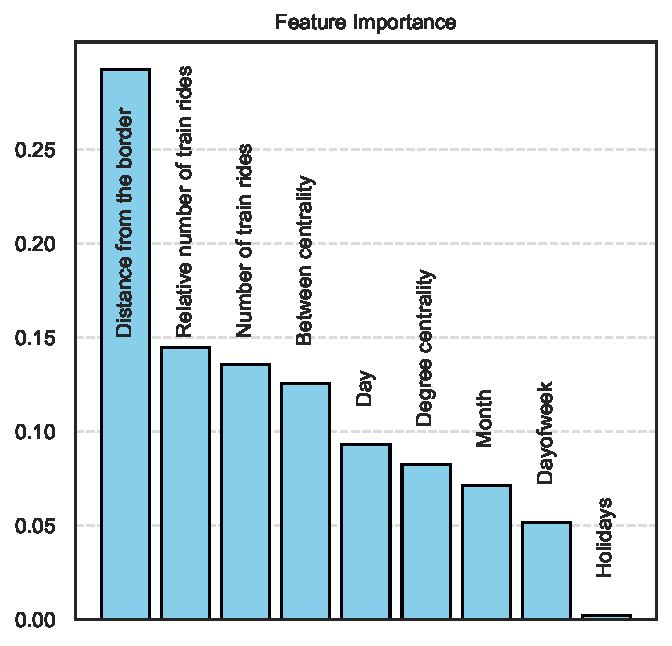
\includegraphics[width=1\linewidth]{fig/plot_JH_feature_importance.pdf}
    \caption{Feature Importance of Random Forest}
    \label{fig:enter-label}
\end{figure}

\subsection{{Centrality Measures}}

After calculating the correlation coefficients related to the delay times between stations, we created edges between two stations if the correlation coefficient was 0.4 or higher. The importance of variables in terms of between centrality was found to be very high, despite being a virtual relationship based on the correlation patterns of delay, rather than a physical connection. 


The betweenness centrality ($C_B(v)$) of a node $v$ in a graph is calculated as the sum of the fraction of all pairs of nodes $(s, t)$, where $s \neq v \neq t$, for which node $v$ lies on the shortest path between $s$ and $t$. The formula for betweenness centrality is given by:

\begin{equation}
C_B(v) = \sum_{s \neq v \neq t} \frac{\sigma_{st}(v)}{\sigma_{st}}
\end{equation}

Here, $\sigma_{st}$ represents the total number of shortest paths from node $s$ to node $t$, and $\sigma_{st}(v)$ represents the number of those paths that pass through node $v$.

This measure provides an indication of how central a node is in terms of facilitating communication between other nodes in the network.

The second centrality measure is closeness centrality. The closeness centrality ($C_C(v)$) of a node $v$ in a graph is a measure of how close it is to all other nodes in the network. It is defined as the reciprocal of the average shortest path distance from node $v$ to all other nodes. According to Ulrik [3], the formula for closeness centrality is given by:

\begin{equation}
C_C(v) = \frac{1}{\sum_{u} d(v, u)}
\end{equation}

Here, $d(v, u)$ represents the shortest path distance from node $v$ to node $u$, and the sum is taken over all other nodes in the network.

Closeness centrality reflects how efficiently a node can communicate with other nodes in the network, emphasizing nodes that are closer to all other nodes.




As argued by Freeman [2], betweenness centrality is one of the most important indicators for a vertex or node because it refers to the extent of the vertex that is structurally central for standing in between others and the vertex can therefore facilitate or impede the transmission of information/goods [1]

betweenness centrality can serve as a very useful tool for rail operators to plan their maintenance schedule because the more ‘central’ stations experience much more stress, resulting in high loadings on its facilities [1]

\subsection{{characteristics of station}}

We considered three factors related to train stations, listed in order of variable importance: distance from the border, the ratio of the given date's train rides to the median of the usual train rides (Relative number of train rides), and the number of train rides. Within the choropleth map (Figure 1 
), it was evident that significant delays occurred near the border. Additionally, the Relative number of train rides measures the likelihood of delays if the train station exceeds its capacity to handle train operations.

\subsection{{Factors related to dates}}

We analyzed the delays based on factors related to dates, including Day, Month, Dayofweek, and Holidays.
??maybe visualization??

\subsection{{Conclusions}}

It is necessary to consider factors beyond simple travel time, such as the operational schedules of other trains and the centrality of specific stations depending on date train system. Additionally, DB operators should consider these factors when deciding train routes and schedules. Centrality metrics and capacity of train stations can be applied to train systems. Future research should explore the interconnectivity between shortest path under the assumption of no delays and probability of delay. 




\section{Limitations}


The delays were computed on a daily average basis, potentially leading to varying results based on different time intervals. Furthermore, our analysis exclusively focused on delay times. A more comprehensive understanding could be achieved by constructing a model that considers both travel time and the probability of delays. The data from the database is incomplete, incorporating only about 35.31\% of the available records for Random Forest model development. Specifically, we considered data from stations with records available for at least 288 days, accounting for over 90\% of this period. Stations with no reported delays throughout the entire duration were excluded from the dataset. 

\bibliography{bibliography}
1. To, W.M. Centrality of an Urban Rail System. \textit{Urban Rail Transit} \textbf{1}, 249–256 (2015).

2. Freeman LC (1977) A set of measures of centrality based on betweenness. Sociometry 40(1):35–41.

3. Ulrik Brandes: On Variants of Shortest-Path Betweenness Centrality and their Generic Computation. Social Networks 30(2):136-145, 2008.
\bibliographystyle{icml2023}


\end{document}


% This document was modified from the file originally made available by
% Pat Langley and Andrea Danyluk for ICML-2K. This version was created
% by Iain Murray in 2018, and modified by Alexandre Bouchard in
% 2019 and 2021 and by Csaba Szepesvari, Gang Niu and Sivan Sabato in 2022.
% Modified again in 2023 by Sivan Sabato and Jonathan Scarlett.
% Previous contributors include Dan Roy, Lise Getoor and Tobias
% Scheffer, which was slightly modified from the 2010 version by
% Thorsten Joachims & Johannes Fuernkranz, slightly modified from the
% 2009 version by Kiri Wagstaff and Sam Roweis's 2008 version, which is
% slightly modified from Prasad Tadepalli's 2007 version which is a
% lightly changed version of the previous year's version by Andrew
% Moore, which was in turn edited from those of Kristian Kersting and
% Codrina Lauth. Alex Smola contributed to the algorithmic style files.
